\subsection{Implementando Una Validación}

% Teniendo definida la notación a usar para la declaración de las arquitecturas objetivo, lo siguiente a realizar era un módulo el cual se encargara de la validación, y construcción, los modelos a usar como referencia. 

Partiendo de la notación definida para la declaración de las arquitecturas de referencia, se realizó la implementación de un cliente que nos permitiera realizar la validación de los archivos de configuración.





La implementación, se dividió en dos partes. Una librería, la cual contiene toda la definición de los objetos definidos en el metamodelo, y será utilizada para la construcción de los modelos en todo el proyecto. La otra parte es un módulo de validación, que se encargará de verificar que los modelos definidos en la notación sean válidos de acuerdo con las reglas establecidas en el metamodelo.

La librería, apodada \textit{StarDuck}, incluye las estructuras para representar las aplicaciones con sus respectivas locaciones y requerimientos de datos. 


Cada clase tiene atributos y métodos que permiten establecer y acceder a sus propiedades de acuerdo con el metamodelo. Por ejemplo, la clase \texttt{Component} tiene atributos como \texttt{name} (nombre del componente), \texttt{component\_type} (tipo de componente), \texttt{components} (componentes internos), \texttt{properties} (propiedades del componente), y \texttt{outputs} (salidas del componente).

El módulo de validación, apodado \textit{Lexical}, se encarga de verificar que los modelos definidos en la notación sigan las reglas establecidas en el metamodelo. Esto incluye verificar que se definan las locaciones y componentes de acuerdo con la estructura del metamodelo, que las propiedades de los componentes sean válidas.

Para implementar la validación, se \textit{parsea} el archivo YAML y se construye una estructura de objetos de acuerdo con las clases definidas en la librería. Durante esta construcción, se aplican las reglas de validación. Si se encuentra algún error, se genera un mensaje de error indicando la ubicación del problema en el archivo de notación. En la figura \ref{fig:LexicalFlow} se puede observar un diagrama de flujo simplificado de este proceso.

\begin{figure}[H]
    \centering
    \caption{Diagrama de flujo del proceso realizado por el módulo \textit{Lexical}}
    \label{fig:LexicalFlow}
    \vspace{2mm}
    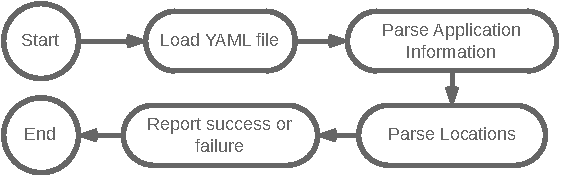
\includegraphics[width=0.8\linewidth]{images/LexicalFlow.pdf}
\end{figure}

El desarrollo de estos módulos, se realizó en Rust. Escogido debido a su capacidad para garantizar la integridad de los datos y prevenir errores comunes, lo que es esencial en un entorno donde la precisión y la confiabilidad son críticas. Además, su ecosistema de herramientas y bibliotecas facilita la implementación eficiente de los módulos de validación y construcción de modelos. \footnote{Todo el código realizado para el proyecto puede encontrase en el grupo de GitHub: \url{https://github.com/ChipDepot/}}

Con la implementación de este módulo de validación, hemos completado la primera fase del desarrollo de nuestra notación y herramienta para describir y validar arquitecturas de aplicaciones de Smart Campus. Ahora podemos avanzar en la implementación de las funcionalidades de comparación y adaptación de modelos, que son parte fundamental de nuestro enfoque de computación autonómica. 


